\documentclass[11pt,a4paper]{report}

% Aberstwyth dissertation LaTeX Template
% Authors: Dr. Hannah Dee (hmd1@aber.ac.uk), Neil Taylor (nst@aber.ac.uk)
% This has been adapted from the Leeds Thesis template and the 
% Group Project template for Computer Science in Aberystywth University.
% 
% All comments and suggestions welcome.
%
% Template designed to be used with pdflatex: it may need alteration to
% run with a different LaTeX engine

% To build document on the unix command line, run four commands:
 
% pdflatex dissertation
% bibtex dissertation
% pdflatex dissertation
% pdflatex dissertation

% you will end up with dissertation.pdf 
\usepackage{mmp}

% the following packages are used for citations - You only need to include one. 
%
% Use the cite package if you are using the numeric style (e.g. IEEEannot). 
% Use the natbib package if you are using the author-date style (e.g. authordate2annot). 
% Only use one of these and comment out the other one. 
%\usepackage{cite}
\usepackage{natbib}

% user-defined packages
\usepackage{titling}
\renewcommand{\subtitle}[1]{%
  \posttitle{%
    \par\end{center}
    \begin{center}\large#1\end{center}
    \vskip0.5em}%
}

\usepackage{tabulary}

% Use the following to selectively exclude chapters
%\includeonly{cover,abstract,acknowledge,declare,chapter1,chapter2}

\begin{document}

% all of the include directives below refer to tex files
% so 
\title{FundFind \\
Exploring scholarly funding opportunities\\
}

% Your name
\author{Emanuil Evgeniev Tolev\\
Degree scheme code: G401\\
Degree scheme title: Computer Science (Inc Integrated Industrial and Professional Training)\\
Degree type: BSc\\
Module code: CS39440\\
Module title: Major Project}

% Your email 
\authoremail{eet9@aber.ac.uk}

\degreeschemecode{G401} %e.g. G400 
\degreeschemetitle{Computer Science (Inc Integrated Industrial and Professional Training)} % e.g. Computer Science
\degreetype{BSc}

\modulecode{CS39440} % i.e. CS39440, CC39440, CS39620
\moduletitle{Major Project} % i.e. Major Project or Minor Project

%\date{6th March 2012} % i.e. the date of this version of the report

\status{Release} % Use draft until you create the release version. Then, change this to Release.
\version{1.0}

%The title and name of your supervisor.
\supervisor{Prof. Reyer Zwiggelaar} 

%The email for your supervisor. 
\supervisoremail{rrz@aber.ac.uk}

\maketitle



 includes cover.tex - to change the content,
% edit the tex file

\pagenumbering{roman}

% This is the front page

\title{FundFind \\
Exploring scholarly funding opportunities\\
}

% Your name
\author{Emanuil Evgeniev Tolev\\
Degree scheme code: G401\\
Degree scheme title: Computer Science (Inc Integrated Industrial and Professional Training)\\
Degree type: BSc\\
Module code: CS39440\\
Module title: Major Project}

% Your email 
\authoremail{eet9@aber.ac.uk}

\degreeschemecode{G401} %e.g. G400 
\degreeschemetitle{Computer Science (Inc Integrated Industrial and Professional Training)} % e.g. Computer Science
\degreetype{BSc}

\modulecode{CS39440} % i.e. CS39440, CC39440, CS39620
\moduletitle{Major Project} % i.e. Major Project or Minor Project

%\date{6th March 2012} % i.e. the date of this version of the report

\status{Release} % Use draft until you create the release version. Then, change this to Release.
\version{1.0}

%The title and name of your supervisor.
\supervisor{Prof. Reyer Zwiggelaar} 

%The email for your supervisor. 
\supervisoremail{rrz@aber.ac.uk}

\maketitle



                        

% Set up page numbering
\pagestyle{empty}

% declarations of originality 
\thispagestyle{empty}

%%%
%%% You must sign the declaration of originality. 
%%%
\begin{center}
    {\LARGE\bf Declaration of originality}
\end{center}

In signing below, I confirm that:

\begin{itemize}
\item{This submission is my own work, except where clearly
indicated.  }

\item{I understand that there are severe penalties for plagiarism 
and other unfair practice, which can lead to loss of marks
or even the withholding of a degree. }
 
\item{I have read the sections on unfair practice in the Students' 
Examinations Handbook and the relevant sections of the 
current Student Handbook of the Department of Computer 
Science.}
 
\item{I understand and agree to abide by the University's
regulations governing these issues.}
\end{itemize}

\vspace{3em}
Signature ............................................................  \\

\vspace{1em}
Date ............................................................ \\

%%% 
%%% We would like to make a selection of final reports available to students that take 
%%% this module in future years. To enable us to do this, we require your consent. You 
%%% are not required that you do this, but if you do give your consent, then we will have 
%%% the option to select yours as one of a number of reports as examples for other 
%%% students. If you would like to give your consent, then please include the following 
%%% text and sign below. If you do not wish to give your consent, please remove this 
%%% from your report. 
%%%
\vspace{5em}
\begin{center}
    {\LARGE\bf Consent to share this work}
\end{center}

In signing below, I hereby agree to this dissertation being made available to other
students and academic staff of the Aberystwyth Computer Science Department.  

\vspace{3em}
Signature ............................................................  \\

\vspace{1em}
Date ............................................................ \\

               

\thispagestyle{empty}

\begin{center}
    {\LARGE\bf Acknowledgements}
\end{center}

I would like to thank my supervisor, Professor Reyer Zwiggelaar for his support and unique approach to the process of producing a major project.

Thanks to Dr. Richard Jensen, Dr. Joanne Walker and Professor Simon Cox for their valuable input in the formative stages of the project.

Furthermore, thanks to all Computer Science Department staff who have taught me over the last 4 years for their patience and being such an inspiration with their varied interests and opinions.

I would like to thank Cottage Labs LLP for introducing me to the Open Knowledge movement, as well as teaching me about most of the major technologies used in this project and agreeing to host a FundFind instance.

Thanks to the Open Knowledge Foundation for striking out and encouraging prototype projects, providing ample inspiration for FundFind.

I would like to thank Research Councils UK, a partnership of the seven UK Research Councils, for all the effort they have put into the Gateway to Research API, consolidating data from seven separate institutions and making it available under an Open license. % Acknowledgements
\thispagestyle{empty}

\begin{center}
    {\LARGE\bf Abstract}
\end{center}

FundFind is a web application which enables scholars, research development officers and postgraduates to share information about funding opportunities. Data about funding opportunities and funding organisations can be submitted, browsed and searched via a mobile-friendly web UI as well as a JSON API. FundFind stores data using an asynchronous approach, which enables the development of small independent modules for automatic funding data harvesting.

The project is a learning excercise, aiming to explore the field of scholarly funding, identifying potential problems with the open sharing of such data. Prototype technical solutions concretise the technical problems. Other types of problems are noted and discussed.                 % Abstract

\pagenumbering{roman}
\pagestyle{fancy}
\fancyhead{}
\fancyfoot[C]{\thepage}
\renewcommand{\headrulewidth}{0 pt}
\renewcommand{\chaptermark}[1]{\markboth{#1}{}}

\tableofcontents   
\newpage
\listoffigures
\newpage 
\listoftables
\newpage

% Set up page numbering
\pagenumbering{arabic}

\setchapterheaderfooter

% include the chapters
\chapter{Background and Objectives}

%This section should pick-up material from your progress report and enhance it based on the feedback and also your additional experience up to now.

%outline the research context or commercial context in which the work was carried out;
%state clearly the objectives of the work;
%review the relevant literature and any similar existing systems;

\section{The Project}
\label{intro-project}
This project is about learning to deal with the field of funding in modern scholarship\footnote{A note on ``scholarship'' - the word and its derivatives are used throughout this text to mean all types of academic work, due to ``science'' being sometimes perceived as exclusionary to the Arts and Humanities fields.} and exploring how it could be opened up, from the point of view of a software developer. It is set within the context of the Open Knowledge field and seeks to add to this field by exploring how scholarly funding can be made more transparent and easier to find for all interested parties.

The main vehicle of learning and main software output is an open-source web application named ``FundFind''. It's a simple crowdsourcing application which allows registered users to share information about funding opportunities under open\footnote{The Open Definition defines ``open'' well \cite{od}.} terms. Its source code is available at \cite{fundfind-src}. Access to submitted information includes a machine-friendly API (Application Programmable Interface).

One of the project features - getting funding data into the datastore - was developed as a separate technical project due to natural low coupling between the main application and this feature. It is called ``Funding Harvest''. Its source code repository is publicly available at \cite{fundingharvest-src}.

\section{Project Aims}
\label{intro-aims}
\begin{itemize}
 \item Learn more about the funding sector and identify user requirements within it. Results presented in \myref{audience} and more concretely in \myref{devprocess-requirements}. The data must be sufficient to enable the creation of a project roadmap for
    \begin{enumerate}[a)]
    \item future research work into the requirements of user groups which were not engaged during this project
    \item concrete development work which would enhance the software built during this project
    \end{enumerate}
  The foundations for this are laid in in \myref{future-work}.
  
 \item Identify how much software it is possible to build by essentially starting and seeing how far it goes in a controlled fashion. The author's own initial lack of domain knowledge about field and technical skill level mean than a fixed feature list is hardly possible. However the progression of features and the final ``shape'' of the FundFind software is discussed in \myref{devprocess-requirements}.
\end{itemize}

\section{Scholarship and Funding}
Scholars need money to conduct research. To be precise, research projects need \emph{additional} money (on top of the investigators' salaries) in order to cover material expenses, travel costs, hiring Research Assistants or providing studentships to PhD candidates and other expenses. 

In other words, established scholars need to look for funding for aims which may be hard to define, for amounts of money ranging from thousands to millions.

Postgraduate-level scholars (candidates, postgraduates, post-doctoral researchers) are also usually looking for a way to fund the next stage of their scholarly career. (Note: undergraduate-level funding was not considered in this project.)

The quintessential problem is that the information about available funding is published in many different places. Usually each funding organisation publishes its own calls for proposals and announces its own studentships on its own website(s) and mailing list(s).

Keeping up with these sources of information becomes quite difficult - so much so, that it takes a significant portion of research development officers' time. Worse still, this is a significant barrier for those looking into a career in academia - the fragmented information can make it difficult to build a mental picture of what the funding in one's chosen field ``looks like''. This leads to a feeling of opaqueness instead of transparency and being overwhelmed - instead of having a clear idea of what it takes to succeed in a chosen field. Sometimes it even leads to accusations of cronyism in distributing funding (e.g. \cite{cronyism1}).

Furthermore, if this process is that difficult for person working in a specific country, then it can easily be estimated that globalisation of scholarship and scholars' mobility is hindered as well.

These problems seem to stem from the fact that the distribution of scholarly funding seems to have evolved over time from a series of changes to more general money distribution in society. This is actually a well-known problem that the software development field has had to deal with - if multiple stakeholders with distinctive interests try to influence the development of a software system, changing its requirements over time, the results can be disastrous.

There is no easy way to track money - where it gets allocated to, what fields (or even topics) within scholarship get funded more than others. Up until November 2012, there was no publicly accessible \emph{centralised} detailed account of historic funding information in the United Kingdom. The Gateway to Research project being implemented by Research Councils UK finally gives a partial (RCUK-specific) overview of historical data.

However, there is still no mechanism of getting \emph{federated, present, current} data about scholarly funding.

Something which allows searching the (vastly) different, \emph{currently available} streams of funding within academia was thus identified as potentially useful by various people interested in the subject.

\subsection{The Value of Openness in Scholarship and Elsewhere}
The Free Software, Open Source and more recently, Open Knowledge (which Open Access is a part of) movements have all demonstrated that the value of information can be greatly multiplied simply by having more people access it, reuse it and even be creative with it (e.g. visualise or summarise). The Open Knowledge Foundation argues this \cite{okfn-vision}. Seminal works like ``The Cathedral and the Bazaar'' \cite{catb} have also argued this.

Governments seem to have grasped the benefits as well. The UK Government has mandated that all research funded with public money (which is a lot in the UK - almost everything through the seven Research Councils) should be published as Open Access by 2014 \cite{guardian-ukgov-oa2014}. It has also funded initiatives such as Open UK governmental data in the form of data.gov.uk \cite{open-uk-gov-data} and the recent Finch report \cite{guardian-finch} \cite{finch}.

The ``Open'' part of ``Open Access'' means more than just throwing the data out there in any form and format. The Open Definition \cite{od} has a lot to say about all aspects of Openness. However, principles \#1 ``Access'' and \#4 ``Absence of Technological Restriction'' are relevant, so it can be seen why the current practice of each funder publishing their own HTML pages is not good enough:

\begin{itemize}
 \item ``The work shall be available as a whole [...] ``As a whole'' prevents the limitation of access by indirect means, for example by only allowing access to a few items of a database at a time.''
 \item ``The work shall be available [...] in a convenient and modifiable form. [...] The work must be provided in such a form that there are no technological obstacles [...]. This can be achieved by the provision of the work in an open data format.''
\end{itemize}

In practice, when applied to scholarly output such as publications, these have been observed by the author to mean ``PDF-s are not going to cut it'', ``You must be able to data mine it''.

\emph{So why not have this for funding data?} Currently, separate HTML pages, weekly e-mails and (sometimes) RSS feeds are all that the Research Councils UK do to publish their funding information. RCUK, in particular, are a publicly funded organisation, and it could be argued that this data belongs to the public. In any case, convincing both public and private funders of the benefits of Open funding data is needed.

Private organisations are not far behind and may in fact be leading the way - one of the largest funders of science in the UK and around the world, the Wellcome Trust, has had a progressive and strict Open Access policy since 2006 \cite{wellcome-oa}.

\section{Audience and High-Level Requirements}
\label{audience}
The potential audience of this project was discovered to be quite varied. It seems multiple stakeholders stand to benefit from more transparent scholarly funding dissemination.

The requirements or potential uses that these users might want to put FundFind to are closely tied to the benefits that come with opening up funding data.

\subsection{Professionals Looking for Funding Group}
\label{audience-professionals}
\subsubsection{Accomplished Scholars}
\begin{itemize}
 \item \textbf{Who}: Academics - lecturers, professors
 \item \textbf{Aims}: Wish to fund future projects
 \item \textbf{Benefits from opening up funding data}: Easier access and search across funding institutions through tools which aggregate funding data; Transparency and accountability of their funding bodies.
 \item \textbf{Possible requirements from FundFind}: Aforementioned cross-funder search; Sharing opportunities with colleagues.
\end{itemize}

\subsubsection{Junior Academics}
\begin{itemize}
 \item \textbf{Who}: Postgraduate candidates, postgraduate students, academics in post-doctoral posts (e.g. Research Associates)
 \item \textbf{Aims}: Wish to find suitable positions to move on with their academic career, e.g. a postgraduate with a PhD will be looking for a post-doctoral position
 \item \textbf{Benefits from opening up funding data}: (More) easily find and compare funding sources
 \item \textbf{Possible requirements from FundFind}: Find funding. To quote a postgraduate candidate: ``I want to do a taught MSc in Astrophysics but I can't afford to self fund. Where can I go and who will pay me?''
 
 Share funding information with peers (e.g. if a candidate for a Computer Vision PhD finds a good PhD studentship call for applications in Bioinformatics, they may well want to forward it to a colleague).
\end{itemize}

\subsubsection{Research Development Officers}
\label{audience-research-officers}
\begin{itemize}
 \item \textbf{Who}: Professionals who find more funding opportunities for scholars
 \item \textbf{Aims}: Wish to record the opportunities they find somewhere and share them with scholars. Also may want to access a list of all opportunities \emph{they} have found over time, so that they can report to their line managers more easily.
 \item \textbf{Benefits from opening up funding data}: Not as many as scholars, unless they are happy to share the opportunities they have found with research officers from other institutions (which they do not always want). However, a system which allows sharing of recorded opportunities with a select subset of users (such as all within the officer's institution) would be welcome as this can allow them to record a funding opportunity once, share it with ``their'' scholars and include it in reports.
 \item \textbf{Possible requirements from FundFind}: Find funding. Share funding with subset of users. See information submitted per user (themselves).
\end{itemize}

\subsection{Funders Group}
Those looking to advertise funding opportunities - Funding Stream and Programme managers at various institutions.

The needs of this group are estimated since funders were not engaged as users at this point in FundFind's development due to time constraints.

\subsubsection{Research Councils in the UK}

\begin{itemize}
 \item \textbf{Who}: Main way of allocating \emph{public} scholarly funding in the United Kingdom.
 \item \textbf{Aims}: Wish to attract the best scholars in their own field, but also look to establish new cross-disciplinary  projects.
 \item \textbf{Benefits from opening up funding data}: Already committed to opening up historical funding data (e.g. Gateway to Research project \cite{rcuk-on-gtr}), would like to advertise current funding data more widely. The benefits are widening impact and increasing the inter- and intra-field interconnectedness of scholarship (scholars can learn about interesting funded projects and people that they didn't know about).
 \item \textbf{Possible requirements from FundFind}: Mostly just search and upload of information. In particular: search for submitted items related to their institution. Bulk upload of opportunities. Control over the ``funder'' profile related to them.
\end{itemize}

\subsubsection{Jisc}

\begin{itemize}
 \item \textbf{Who}: Used to be known as ``Joint Information Systems Committee'', but have decided to rebrand \cite{jisc-rebrand}. The old name of this public organisation reflects their purpose quite well - helping the adoption of digital technology in research and teaching in the UK.
 \item \textbf{Aims}: Wish to attract talent to work on scholarly infrastructure in the UK, i.e. give their aims and projects more exposure. Scholars rarely choose scholarship infrastructure as their main field.
 \item \textbf{Benefits from opening up funding data}: Have always wanted wider reach, as well as vigorously supported Open Data. Have a lot of funding opportunities, both minor and larger ones. Would like to advertise them better.
 \item \textbf{Possible requirements from FundFind}:  The same as RCUK. In addition, however, they might wish to actually use FundFind's data in other projects - in other words, they might be an interested API consumer.
\end{itemize}

\subsubsection{Charities, Trusts and Others}

\begin{itemize}
 \item \textbf{Who}: Various charitable Foundations, Institutes, Endowments and so on which fund scholarly activities (e.g. the Wellcome Trust \cite{wellcome-trust}, Shuttleworth Foundation \cite{shuttleworth-foundation}, Knight Foundation \cite{knight-foundation}).
 \item \textbf{Aims}: Simple - want the best scholars competing for their money (at least the portion dedicated to conventional research).
 \item \textbf{Benefits from opening up funding data}: Need to reach more scholars to build up an ever-improving pool of applicants (in terms of quality). Also, as private institutions, would like to demonstrate greater transparency with their funding dissemination and allocation as part of their efforts to prove they are doing it effectively.
 \item \textbf{Possible requirements from FundFind}: Same as RCUK.
\end{itemize}

\subsubsection{Commercial Organisations}

\begin{itemize}
 \item \textbf{Who}: All companies which perform R\&D activities. Famous UK examples include Rolls-Royce \cite{rolls-royce} and IBM \cite{ibm}.
 \item \textbf{Aims}: The ones with large enough R\&D budgets to get involved with scholars usually invest in whole laboratories and centres. When they do share effort and money with research institutions, they do have to search for the ``best scholars'' to collaborate with. The smaller ones may have a problem however - they may only need external help with R\&D intermittently and thus may not have a ``constant'' audience of scholars following their every move since they would not be allocating funding all the time.
 \item \textbf{Benefits from opening up funding data}: Greater transparency of funding allocation, potentially greater audience if a federated scholarship funding source like a popular FundFind instance does come into existence at some point.
 \item \textbf{Possible requirements from FundFind}: Same as RCUK.
\end{itemize}

\subsection{Analyst Group}
\label{audience-analyst}
Those looking to analyse scholarly funding - how it is allocated and/or spent.

A hackday in the middle of March which focused on the Gateway to Research project provided insight into the usefulness of certain initially planned features and inspired new ideas. The main audience of the hackday was this group. The GtR is an attempt to get the seven UK Research councils to publish historical funding data - who got funded, grant codes, who worked with whom, any related publications \cite{gtr}, etcetera via a web interface and a RESTful API. GtR is quite similar to FundFind, except that it relates to \emph{historical}, not current funding information, and of course contains a lot more information than FundFind is currently scoped to hold.

\begin{itemize}
 \item \textbf{Who}: Software developers, journalists and others interested in Open Knowledge and visualising data for the purposes of transparency or advancing the digital economy \cite{okfn-vision} The author is included in this group. Other interested parties are analysts, bloggers and the general public.
 \item \textbf{Aims}: Want transparency and accountability. May want to visualise how scholarship money is being spent or otherwise help society engage with scholarly spending.
 \item \textbf{Benefits from opening up funding data}: Open Data essential for re-use for their aims. Usually do not have first hand information about what happens behind closed doors when funding is distributed and used by universities. Think that this is strange, since often both funder and fundee are public sector organisations / employees.
 \item \textbf{Possible requirements from FundFind}: 
\end{itemize}

There is another group which belongs here - politicians. They may wish to demonstrate accountability and good decision making. Despite the fact that they are not usually known to readily embrace new technological solutions, they do do it when the advantages (at least from a Public Relations perspective, if no other) become clear. For example, the UK government more or less suddenly embraced Open Access for all publicly funded research \cite{guardian-ukgov-oa2014}.

\subsection{Focusing on Certain Audience Groups}
\label{focus-groups}
Satisfying the requirements of all user groups is more suitable for a larger, better-resourced project than this one.

This project will focus on the first group of users'' meaning \myref{audience-professionals}. The main reasons are still ``time constraints and ease of access to such users''. However, the \myref{audience-analyst} was also taken into account. This was partly because the success of a technological project just has to include other developers, especially when it is an open-source project. On the other hand, the author is part of this group and day-to-day interactions create unavoidable bias, especially when they include learning (how to use technologies relevant to FundFind) and feedback on the very project being developed.

As stated previously in the Progress Report, FundFind does have an open machine-ready to communicate with other software - an Application Programmable Interface (API). In terms of concrete people within this group, Cottage Labs LLP \cite{cl} still find value in the project and will probably help to take it further after the current development as a piece of course work ends.

In addition to the The Open Knowledge Foundation \cite{okfn-vision}, to whom the project will be presented after it is finished and feedback will be asked for, the Gateway to Research technical team will also be contacted about possibly building a stronger relationship with FundFind. They might be interested in its use of the data provided by their API to make suggestions of interesting projects (to look at) to scholars. Furthermore, they handle \emph{historical} funding data, whereas FundFind handles \emph{current} funding data. Convincing the Research Councils UK to provide the same uniform interface to their \emph{current} funding data as they are to their \emph{historical} data with the GtR project would be a great boon to the Open Knowledge movement.

\section{Existing Works}
\label{existing-works}
There is no single piece or combination of pieces of software which enables the identified audience to do what this project would allow them to do upon completion, to the best of the author's knowledge.

Related Open Knowledge projects are still as relevant as at the beginning of the project, in particular the Open Knowledge Foundation ones at \cite{okfn-labs} and \cite{okfn-github}. \myref{design-rationale} notes individual projects which informed FundFind's technical design in some way.

The FundFind codebase was initially based entirely on the IDFind project \cite{idfind}, which is available under the MIT license \cite{idfind-src}. Cottage Labs LLP and the author started it during the DevXS 2011 conference \cite{devxs}. IDFind was a good place to start, since the project's context (Open Knowledge, interested parties) is similar, so a similar set up and technologies could be used to accelerate the initial development.

\section{Licensing}

FundFind is licensed under the MIT license, like its parent IDFind. This is a permissive license which should facilitate the widest possible use and reuse of code. Moreover, there is little reason to place particular restrictions since the target Open Knowledge / Funding fields are narrow enough and there isn't really any open-source software which sits at the intersection of the two.

\subsection{Contributions}

Contributions through FundFind's user interface (crowdsourcing) are licensed under the Creative Commons Attribution (CC-BY) \cite{cc-by-3} license, version 3.0 (latest at time of writing). This was chosen after considering a multitude of other licenses. In the end, the new Budapest Open Access Initiative recommendations and the Open Definition \cite{od} recommending CC-BY informed the choice.

This license only applies to publicly visible (shared with the world) submissions. For now, it is not possible to share funding information only with certain users or groups - therefore, the license applies to all crowdsourced contributions. Proper access control was too costly to implement in light of more important / core features which would enable the system to at least act as a prototype for completely open sharing, before moving on to the more complex role of a virtual shelf of funding opportunities.

The contributions license does not apply to data which has been harvested from data sources (like funders' websites or RSS feeds) automatically. The owners of the data would have to give written consent for Funding Harvest to harvest their data and publish it as CC-BY (or, better and more likely - publish it as CC-BY themselves). Funding Harvest is only a tool which, in combination with FundFind, is meant to showcase the benefits of having funding data open, thus convincing data sources to publish data more openly. It is not a tool to infringe on the copyrights of others, although it can be used as such. This is true of any software which does page scraping or even just consumes and records RSS feeds.

Most records in FundFind's datastore denote the license they can be used under. If a record does not have a |license| field (user accounts do not, for example), then the default (restrictive) copyright rules apply to that data.
%\addcontentsline{toc}{chapter}{Development Process}
\chapter{Development Process}



\section{Introduction}
%Introduce the specific model that you chose to use. 
% You need to describe briefly the life cycle model that you used. Do not force your project into the waterfall model if it is better described by prototyping or some other evolutionary model. You do not need to write about all of the different process models that you are aware of. Focus on the process model that you have used. It is possible that you needed to adapt an existing process model to suit your project; clearly identify what you used and how you adapted it for your needs.


The project used an evolutionary prototyping approach. There were two phases:
\begin{enumerate}
 \item requirements gathering; building the basic application structure, in particular submission of information; investigating appropriate technologies
 \item building the features from the initial feature list feature-by-feature; some were dropped due to difficulties with them or higher priority features - final list arrived at through this iterative process
\end{enumerate}

An Agile, iterative approach to the development of the software was initially chosen. It turned out that the approach did not fit the project / author / users context. In particular:

\begin{enumerate}
 \item The initial approach was actually not Agile to begin with (a problem of understanding what Agile actually entails).
 \item Agile requires a certain level of understanding of the technology (developer's side) and problem the software is solving (``customers''' or users' side).
\end{enumerate}

The length of the requirements gathering phase and the complexity of developing the most important features was initially underestimated. Analysis of the intermediate outputs and measurement against the initial aims suggested that a different scope was necessary. The new goals required a different approach, but that alone would not provide an answer as to what FundFind should have aimed for while remaining realistic.

Concentrating on and discussing the original goal of the FundFind project with interested parties proved fruitful. The overarching aims of ``learning about scholarly funding'' and ``prototyping a solution for sharing this information'' resulted in a leaner, more focussed set of requirements to work towards. Since work on the code had started and a basic web application was running, it was most appropriate to enhance this and peruse the chosen datastore's unique characteristics to add new features while retaining simplicity. This approach in the second phase of the project was essentially faster evolutionary prototyping (compared to the first phase), mostly due to building better understanding of the technologies involved and insufficient time to deliver all features on the list.

\subsection{Project management tools}
\label{pm-tools}
A project management piece of software suited for Agile approaches was chosen to manage this project and was used successfully throughout: PivotalTracker. The project's progress and a list of features (in priority order) has been publicly available at \cite{pm} throughout the project's current lifespan (October 2012 - April 2013).

A private source code version control repository was set up with GitHub \cite{github}. It is only private due to several concerns:
\begin{enumerate}
 \item The licensing status of the IDFind project which FundFind was forked off, was unclear. In fact, with no license statement anywhere in the repository, the default copyright rules apply and FundFind could not have been legally based on IDFind without explicit written permission from the authors. However, since IDFind's only contributors were Cottage Labs LLP and the author of FundFind, this did not delay FundFind's development. Nevertheless, IDFind's licensing status was not cleared up until April 2013.
 
 \item There were concerns about the quality of FundFind's code and the repository. GitHub is home to enough orphan repositories which are all almost empty or without proper licensing, either of which makes the project useless in terms of its Open Source aspect.
 
 \item It wasn't quite clear whether the code could be released during the official timeline of the final-year Major Project module at the author's institution. One of the main ideas in open-sourcing code is that others can contribute to it, but that would have significantly complicated matters in terms of reviewing the final version of the code. Cottage Labs LLP would like to contribute, but agreed that they are busy enough at the moment to look at the codebase after the 26th April 2013 (by which time a copy of FundFind's codebase would have been handed in).
\end{enumerate}

Furthermore, a private repository holding all of the other outputs of the author's Major Project (Outline Specification, Progress Report, presentation files, this document and so on) was set up purely for back-up purposes.

\section{Evolution of the Development Process}
Initially, Agile practices such as Pair Programming \cite{pairprg}, full Scrum \cite{Scrum} and Feature-Driven Development were deemed unsuitable since they are aimed at groups of developers. Behaviour-Driven Development (with Cucumber \cite{cucumber}) was considered, but requires more commitment from the users - they need to learn an English-like domain-specific language which describes how the system is going to behave which didn't sit well with assumption \#2 above and turned out to be the right decision as that assumption proved correct.

Thus, initially, with no methodology fitting the precise needs of the project and the Agile Manifesto \cite{agile-manifesto} in mind, a methodology of an Agile \emph{character} was planned, using the Extreme Programming lifecycle as a base \cite{xp-lifecycle}. The idea was to use ideas such as Release Planning (plan a set of features), Iteration (develop in small increments) and Stories (described above).

The basic steps which were defined were:
\begin{shadequote}
\begin{enumerate}
	\item Meet with a variety of potential users from the chosen user group (\S\ref{focus-groups}), trying to pick them so that each one has a different professional perspective on scholarship.
	\par\emph{Emanuil Tolev in FundFind Progress Report \cite{progress-report}}
	\setcounter{tmpc}{\theenumi}
\end{enumerate}
\end{shadequote}

This worked well, with candidate postgraduates, postgraduates, research assistants (post-doctoral), lecturers and developers all agreeing to give a bit of their time. The meetings were not as regular as initially hoped (1 per month with each user) due to users' commitments, author's committments and a particular characteristic of this project.

Looking at requirements presented in \S\ref{audience}, it is easy to see that the basic searching and sharing of opportunities were two \emph{really} important functions. Sharing is used to different ends by research officers, lecturers, postgraduates and funders, while searching is useful for different reasons to pretty much everybody. However, getting timely feedback from all target users was not considered to be possible - and that is required for iterative development. It was actually considered (and turned out to be - \S\ref{impl-hard-basics}) difficult enough to produce a prototype which made progress in satisfying the initial requirements of \emph{multiple} groups. Thus, meetings essentially happened at the start at the project (October, November, December) and at the end, in March and April, since most of the time inbetween was spent getting those two important features right. Advanced functionality was planned in March and developed in April and is described below in \S\ref{final-reqs}.

\begin{shadequote}
\begin{enumerate}
	\setcounter{enumi}{\thetmpc}
	\item Define \emph{and prioritise} the functionality of the project with each user in the form of the ``stories'' mentioned above. Record the results using the chosen project management tools (\S\ref{pm-tools}).
	\par\emph{Emanuil Tolev in FundFind Progress Report \cite{progress-report}}
	\setcounter{tmpc}{\theenumi}
\end{enumerate}
\end{shadequote}

%This turned out to be a really good idea 

\begin{shadequote}
\begin{enumerate}
	\setcounter{enumi}{\thetmpc}
	\item Release planning - prepare an initial timeline of which project features are to be released when and denote ``release points''. This work can be repeated as required - the order and the features themselves might change on the basis of user feedback over time (this is how Agile projects try to deliver more value by responding to changing requirements). The total size of the work and the size of each feature will most probably remain the same. This piece of work produces the ``Project Timeline'' and the current version is included in \S\ref{timeline}.
	\par\emph{Emanuil Tolev in FundFind Progress Report \cite{progress-report}}
	\setcounter{tmpc}{\theenumi}
\end{enumerate}
\end{shadequote}

\begin{shadequote}
\begin{enumerate}
	\setcounter{enumi}{\thetmpc}
	\item Iterate - every week is a self-contained unit of work consisting of coding, documentation and write-up work. Before starting to code each week, break up that week's story into tasks so goals can be tracked more effectively and there is something to be accomplished each day.
	\par\emph{Emanuil Tolev in FundFind Progress Report \cite{progress-report}}
	\setcounter{tmpc}{\theenumi}
\end{enumerate}
\end{shadequote}

\begin{shadequote}
\begin{enumerate}
	\setcounter{enumi}{\thetmpc}
	\item Repeat items 1 and 2 - meaning regular meetings with previously chosen users - one per user per month, demonstrate the latest features and record the feedback.
	\par\emph{Emanuil Tolev in FundFind Progress Report \cite{progress-report}}
	\setcounter{tmpc}{\theenumi}
\end{enumerate}
\end{shadequote}
	


% Within the coding part of each iteration, Test-Driven Development is employed using both unit and integration tests (the latter via browser automation with Selenium \cite{selenium}). This will be the evidence (on a basic technical level) for the ``correctness'' of the software. A basic form of Continuous Integration \cite{ci} will also be used - the Jenkins \cite{jenkins} software is currently being evaluated for the job. It basically runs all automated tests continuously, helping to detect regressions in code quality.
% 
% This methodology makes for a considerably simpler lifecycle than the Extreme Programming one (a visualisation of which can be accessed at \cite{xp-lifecycle}). This is intentional as there are only about 11 (potentially 13) weeks which allow for programming work as can be seen in \S\ref{timeline}.
% 
% The length of one iteration will be one week. Considering the tight deliverable deadlines (see \S\ref{timeline}), this will keep work on the project focused and will force the definition of user stories of a manageable size.

%Agile approaches usually \emph{avoid} defining ``size'' - how long it will take to implement a story. Rather the complexity of each story is estimated using \emph{arbitrary} numbers (some people prefer to use larger/smaller animals) - how difficult it is to implement that story relative to other stories. If a story seems too \emph{complex}, it needs to broken up. This project uses the Fibonacci number sequence \cite{fibonacci} and ``too complex'' is a complexity estimate of more than 3. Previous experience with the technologies involved has also helped provide a link between complexity and ``how much time will it take'', thus helping enforce a maximum of 1 week to complete a story and add value to the software.

% Saying ``actual features being implemented could change due to the Agile project development methodology'' as the Progress Report did does not make the approach Agile, as Agile is not a stick that one uses to prune excessive features at will - it is an approach that the developer sticks to.

\section{Modifications}
%Did you have to modify the model to suit a one-person project. If so, what did you change and why? 
In the Progress Report features were planned and \emph{scheduled} in a timeline before development took place, but that is \emph{not} the Agile way at all.

\subsection{What is Agile?}
Agile is about getting work done in an iterative fashion so that there is always working software for the users to use. Estimates in Agile are about effort, complexity and risk. Estimates are also \emph{relative} - when new features are added to the project scope, they are estimated in comparison to previously added ones. (For a commonly used estimation points scale and more elaboration on Agile estimation, see \cite{agile-estimate}.) If numeric points are used for the estimation, the project ends up with several hundred / thousand points worth of features.

Since those are prioritised by the customer/users, work can then start. What Agile teams seem to do is to essentially see how quickly they get through work - how many points they go through per week, which is called the ``velocity'' of the team.

Only then is it possible to estimate how long all of the initially requested features will take to develop - by taking into account their ``size'' (relative to each other) and the team's abilities. Taking the total project size and dividing it by the weekly velocity gives a rough idea of how many weeks it would take to complete all requested features. Let this be |time_required|.

If |time_available < time_required|, then the scope of the project simply has to be limited, i.e. features have to be dropped, and this only becomes clear once velocity is established (so at least a few weeks after development has started). In other words, however many features there \emph{turns out} to be time for in the development process are \emph{what gets done}, which is why there is so much emphasis on having the users involved - prioritising the functionality themselves.

\subsection{Is it Agile?}

FundFind's Progress Report \cite{progress-report} stated that an Agile-like methodology had been chosen - the main concept being user stories which allow capturing user requirements very quickly in an informal way.

Having a list of desirable features is great, having a schedule of which one will be delivered when - not so much. The point of Agile is taking the specifics of the development team and users' knowledge (and specificity of their desires) into account. A fully pre-defined plan - even one informed by meeting users, such as in this case - disregards all of this and does not conform to Agile's flexibility requirements. (Responding to change better than more conventional approaches is usually one of the first touted benefits of Agile approaches.) 

Figure \ref{fig:timeline} presents that initial plan.
\newpage
\begin{figure}[H]
\centering
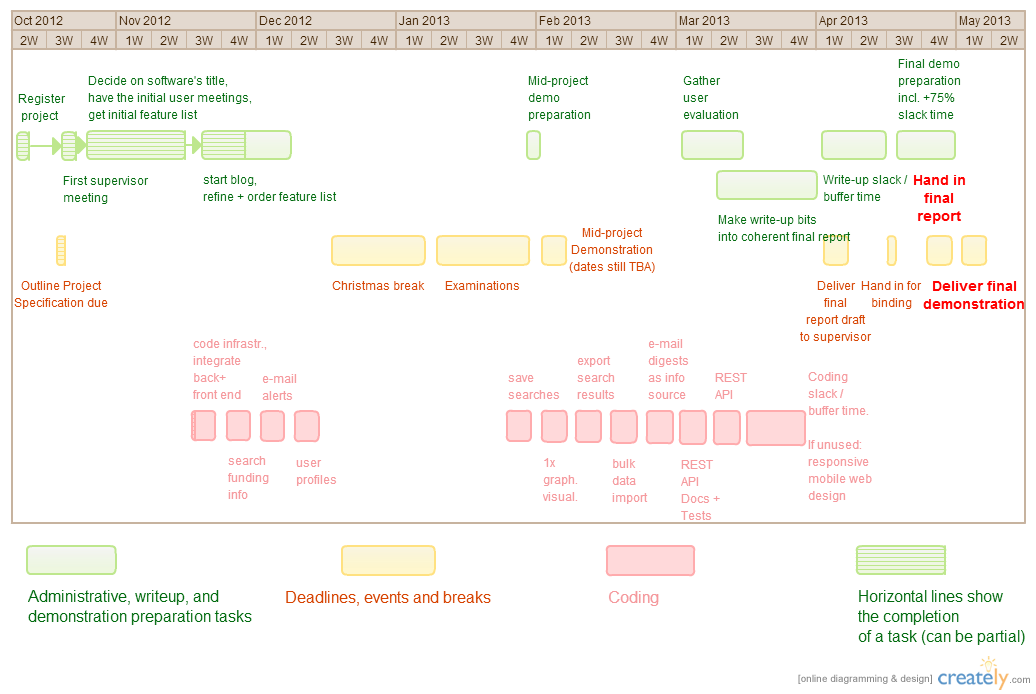
\includegraphics[height=0.6\textheight,angle=90]{Images/timeline.png}
\caption{FundFind initial timeline}
\label{fig:timeline}
\end{figure}
\newpage

\subsubsection{Underestimation}

The main reasons for choosing Agile were
\label{agile-reasons}
\begin{enumerate}
 \item Agile's perceived advantage in pinning down changing requirements.
 \item Less formal communication with the users, who are all busy professionals. It was assumed they would not have sufficient time for writing functional specifications, even in collaboration with the author (as can sometimes be assumed in industry).
 \item Linked to the user communication reason was a concept which many Agile methodologies used - user stories. These are short sentences (or rarely, paragraphs) which describe a single piece of functionality - a single ``thing'' that the user wants to do with the system.
\end{enumerate}

However, it turned out that both the complexity of the scholarly funding field and the author's ability to concretise fuzzy requirements, as well as their technical skill had been underestimated (elaborated upon in Chapter \ref{eval}). The fact that requirements had to be gathered and concretised is not unusual in Agile, but playing both developer and user was a problem. 

Neither did users have enough time to be properly involved throughout the project, nor did the author have enough domain knowledge to understand the requirements and develop quickly enough \emph{in order to get the users involved} in the way in which Agile understands involvement.

This conclusion and the process of arriving at it, ultimately, are the reason why the initial Agile-like development process was deemed unsuitable and why the project's progress is split so starkly into two phases as per Figure \ref{fig:new-process}.

The initial reasons for devising an Agile-like process (above) proved to (mostly) be steps in the right direction, however:
\begin{enumerate}
 \item The flexible requirements reason did not work out so well since it turned out the requirements did not change or need to change. Issues with funding data have been present for a while and a system which tries to prototype fixes through Open Data for some of them needs (a) developer(s) who know these issues inside out. of course, the requirements gathering can still be done in an Agile way, but needs to be mostly completed before development starts. Defining the problem, in this case, had to come before solving it.
 
 It could be argued that this was only a problem since the developer was also the ``initiator'' of the project (i.e. had to play user a lot more than usual). If a particular funder, Higher Education Institution or an organisation like the Open Knowledge Foundation wanted a project like this done, they would already know of certain problem characteristics - such as \emph{particular} drawbacks of having so much funding data ``closed''. Then, more targeted exploration could be done and technical development would also have more precise targets to meet.
 
 This is, in part, what caused the development process to look a lot more like \textbf{evolutionary prototyping} with a lot of requirements gathering between the prototype versions in Figure \ref{fig:new-process} rather than an Agile iterative approach.
 
 \item The assumption that users won't have time for anything but informal problem specification turned out to be correct. Thus, the ``stories'' concept proved to play an important role when gathering requirements from the target audience in short meetings, on the go or at hackdays.
 
 \item The project's stories have been publicly accessible at the PivotalTracker management tool continuously throughout the exploration phase of the project which was used to record the aforementioned informal requirements. The ``Icebox'' still contains the list of features as prioritised by the various users who have been consulted during the exploration phase.
\end{enumerate}

\section{Requirements}
\label{devprocess-requirements}
% In most cases, the agreed objectives or requirements will be the result of a compromise between what would ideally have been produced and what was felt to be possible in the time available. A discussion of the process of arriving at the final list is usually appropriate.

% not everything described in audience could be done

In this case, the project's requirements (in a suitable share-able form) are actually part of the expected project output, as one of the main aims is to learn about the scholarly funding field and identify needs.

\subsection{Requirements Gathering}
The process was essentially arranged 0.5h and 1h meetings with interested users and talking about

\begin{enumerate}
 \item what features they might find useful in a system such as FundFind and how the current list (as of the meeting) should be prioritised
 \item about the scholarly funding field in general (in an attempt to get everybody's point of view and be able to learn what their needs might be from the differences in the way people approached the field)
 \item about their role in this field (if any) in a further attempt to gather user needs information that might not have been otherwise articulated
\end{enumerate}

The results of each meeting fed into the next one due to item \#1. The final result is the list of requirements below.

It was quite difficult to get users to articulate what they need - FundFind does not match their current workflow, so there was a disconnect between the way they thought and the questions asked (e.g. ``saving searches'' means nothing to somebody who does not use a particular interface or system to search - it is akin to asking them if they save a copy of Google's results page for later use). This is the reason items \#2 and \#3 made it into the interview methods above after the first meeting.

Both of these methods required significant interpretation on the interviewer's side to produce useful results. While they certainly worked for generating new feature ideas, there wasn't much guarantee that those ideas would match the users' actual needs. Interpreting without much domain knowledge was one of the most difficult parts of the whole project.
% process - meetings etc.; any difficulties
% results - intermediary list - below

\subsection{Initial Requirements}
\label{initial-reqs}
The initial requirements were informed by the general needs of the various audience groups (\myref{audience}).

They are listed below alongside changes which were made (kept/dropped/changed/changed priority). Further discussion on the lessons learned and future work enabled by the dropped features is presented in \myref{future-work}. Features which went through major changes are discussed below in \myref{new-reqs}.

In \textbf{order of importance}:
\subsubsection{Search For Scholarly Funding Opportunities}
\begin{itemize}
 \item \textbf{Why}: It's the implementation of one of the main project goals - making funding information discoverable. Every single audience group needs it in one way or another.
 \item \textbf{Priority rationale}: All users decided it was a top-priority feature, very much the main point of a system like FundFind.
 \item \textbf{Decision}: \textbf{Kept as-is}. No information suggested that this had actually become any less important than when the project started, and although the project goals changed when it became clear how much expertise was needed to actually do everything well, this was still an important software feature.
\end{itemize}

\subsubsection{Submit Information About A Scholarly Funding Opportunity}
\begin{itemize}
 \item \textbf{Why}: In a similar vein to searching for such opportunities, multiple audience groups need it, albeit for different  reasons (a funder might want to make their opportunity more discoverable, while a PhD candidate can just share a good opportunity with their peers).
 \item \textbf{Priority rationale}: Core to the crowdsourcing functionality of the project. Actually incentivising users to do this is a different matter entirely. That is part of the point of FundFind though - through providing the capability to share, it gives a reference point to related conversations and feedback, (hopefully) allowing developers to understand why the various users do not want to share funding information.
 
 of course, this requires the search functionality to be present to provide great value to the project and is thus still second.
 \item \textbf{Decision}: \textbf{Kept as-is}, for the same reasons as the feature above.
 
\end{itemize}

\subsubsection{Submit Information About Funders}
\begin{itemize}
 \item \textbf{Why}: At the start of the project there were concerns that the various funding opportunities are vastly different in their purpose, format and thus, the data available about them. In order to alleviate this expected problem, this idea was presented to users and was found to be reasonable.
 
 In essence, if the funding opportunity data isn't good enough, a catalogue of funders would still be quite valuable. It was presumed to include some information to let the user search for an appropriate funder - like tagging the funders, or describing their interests.
 
 The idea actually came from a different Open Knowledge-related project called ACat (\textbf{A}cademic \textbf{Cat}alogue) \cite{acat} - an attempt to mine all information on all academic publishers, their journals \emph{and articles}. Even though ACat was just a hackday idea and hasn't evolved much since June 2012, it clearly showed the importance and value of having a list as simple as ``all UK academic publishers''.
 
 \item \textbf{Priority rationale}: Similar reasons to the feature above for this one to be so high up in the list in terms of crowdsourcing functionality. Its importance is very much tied to submitting information on funding opportunities - the more difficult it is to reconcile data from multiple sources (within the current scope), the more important this becomes.
 \item \textbf{Decision}: \textbf{Kept as-is}, for the same reasons as the feature above.
\end{itemize}

\subsubsection{Create Profiles}
\begin{itemize}
 \item \textbf{Why}: Submissions of data could not be anonymous \emph{to the system} - the submitter has to be authenticated and logged in some way, otherwise the submission forms will likely become the target of spam bots. It also helps with data quality, although admittedly on a very basic level - essentially, if a user is bothered to register, they are less likely to submit random junk into the system.
 
 This feature could include more than a username and a password however - it could include declaring research interest keywords and affiliations (the latter having been recorded as a separate feature at user meetings - see below).
 \item \textbf{Priority rationale}: Really desirable to enhance the basic functionality described above, but not as vital as actually having said functionality work in the first place.
 
 Other features which did not fit in the initial timeline at all but were earmarked for inclusion into a ``Future work'' section also require this (for example, research officers' reports \myref{future-research-officers-reports}).
 \item \textbf{Decision}: \textbf{Kept. Not much changed} except ``could include more than username and password'' became ``includes more...'' as no particular difficulties arose during the design or implementation of these additional fields.
\end{itemize}

\subsubsection{Visualise Data}
\begin{itemize}
 \item \textbf{Why}: It was thought that the Analyst audience group \myref{audience-analysis} would have an interest in this as it might spark other ideas about visualising funding data. Furthermore, scholars themselves might have had use for the result of the analysis - such as knowing how much their field is being funded at the moment.
 \item \textbf{Priority rationale}: Showcased the benefits of opening up funding data, which is one of FundFind's goals.
 \item \textbf{Decision}: \textbf{Dropped}. This turned out to be a little ill-defined. It embodied the quintessential software development problem of trying to predict what users want without actually knowing or being able to venture a good guess. The initial reasons as to why a visualisation might be useful are still true, of course, but it turned out developers who had done other Higher Education work understood the benefits of visualising such data quite well. Similarly, scholars could tell how well their field was funded just by looking at the data - the problem being that creating a visualisation that hid data appropriately and thus decreased cognitive load or increased insight was actually quite difficult. Representing the data in some much simpler visual way was not as hard, but also far from useful for people used to interpreting textual and numeric data. These insights were gained mainly during the Gateway to Research hackday (\myref{audience-analyst}).
\end{itemize}

\subsubsection{E-mail Alerts}
\begin{itemize}
 \item \textbf{Why}: Requirements gathering showed users using e-mail alerts / digests to receive the newest calls from funders. Thus, FundFind should probably offer a similar service as it federates such information.
 \item \textbf{Priority rationale}: Simply get users to use FundFind. With it, they would be getting the same information they could elsewhere, so this is just covering for value proposition \#2 from \myref{value-propositions}.
 \item \textbf{Decision}: \textbf{Dropped}. Turned out data - getting data - was more important than the gimmicks of managing data. This is where FundFind's role as a prototype and a limited vehicle of learning came into play.
\end{itemize}

\subsubsection{Saving Searches}
\label{reqs-saving-searches}
\begin{itemize}
 \item \textbf{Why}: In a similar fashion to e-mail alerts, this was thought to be important as it allowed for better management of data and reduced repeated search effort.
 \item \textbf{Priority rationale}: Part of value proposition \#3 - additional features. Other features such as e-mail alerts actually could be implemented more easily after this one is done - however, users did not think it was such a high priority. It also turned out that searches can already be shared just by copy/pasting the URL of the search page (\myref{impl-facetview}.
 \item \textbf{Decision}: \textbf{Dropped}. Similarly to e-mail alerts, it turned out data is the first thing to get into the application and leave enhancements for later.
\end{itemize}

\subsubsection{Harvesting Funding Data From E-mail Digests}
\label{devprocess-feats-email-harvest}
\begin{itemize}
 \item \textbf{Why}: This is one of the features which actually deal with importing data, fulfilling part of FundFind's core mission of federating funding data.
 \item \textbf{Priority rationale}: The importance of this was downplayed by the author - users did not have much to say on it, since they did not particularly care for the details of how FundFind was going to get its data, as long as it had some and they could use it.
 \item \textbf{Decision}: \textbf{Changed}. This is a good idea - however, all the information turned out to be available in machine readable formats (for the funders which were considered). It was also technically quite challenging (\myref{impl-email-parse}).
\end{itemize}

\subsubsection{Tagging Research as "Potentially of Interest to" Users and Groups}
\begin{itemize}
 \item \textbf{Why}: Part of showcasing the benefits of opening up and sharing funding data - enables scholars and research development officers to target the sharing of opportunities. May also enable funder representatives to target their funding calls better, although care has to be taken since the two sides of the ``advertisement'' may well have different goals.
 \item \textbf{Priority rationale}: This is a nice feature, but builds on profiles, search and submissions working, so just has to be done after them.
 \item \textbf{Decision}: \textbf{Kept as-is}.
\end{itemize}

\subsubsection{Specify Affiliation and Interests}
\begin{itemize}
 \item \textbf{Why}: This is actually the ``other end'' of tagging research - specifying where the user works (institution, research group, country) and what field the user works in (interests) enables the usage of the tags associated with research data.
 \item \textbf{Priority rationale}: Similarly to tagging research, this feature builds on everything before it, clearly part of value proposition \#3.
 \item \textbf{Decision}: \textbf{Kept as-is}.
\end{itemize}

All initial features described below were lower priority or in some way optional in relation to the main aims of the project.

\subsubsection{Responsive Mobile Web Design}
\begin{itemize}
 \item \textbf{Why}: FundFind is all about sharing data, thus it made sense to let people share in as many contexts as possible. The Design Rationale \myref{design-rationale} elaborates further on this feature, which is actually a UI design characteristic. It was also of personal technical interest to the author - responsive web user interfaces are everywhere in the Open Knowledge field. Some work better, some worse, yet one thing is clear - learning how to develop them is important. Preliminary research also showed that implementation might not actually be that difficult (\myref{impl-mobile}), especially with a more lax testing strategy (\myref{testing-mobile}).
 \item \textbf{Priority rationale}: As technically nice as this is, it was certainly not prioritised highly by users. Therefore, it was given a lower priority than the main functions of the application.
 \item \textbf{Decision}: \textbf{Kept as-is}.
\end{itemize}

\subsubsection{Bulk Funding Opportunity Data Import}
\begin{itemize}
 \item \textbf{Why}: Importing funding information records one-by-one can get quite boring, time-consuming and tiring - all the characteristics of a task that is ready to be automated. This was mainly conceived as a feature for the Analyst audience group (\myref{audience-analyst}), specifically more advanced users who might want to use the software itself and load it up with data they are interested in - not the data all other users have shared on the public FundFind instance. This also includes potential contributors to the code. Another potential target was funder representatives, who may have access to funding opportunity information from their organisation in a structured format and would rather just upload it than copy/paste the records one-by-one.
 \item \textbf{Priority rationale}: This feature has quite a narrow focus - a (very) narrow subset of the audience of the project.
 \item \textbf{Decision}: \textbf{Dropped} - it was just really of very limited use. Even backing up the data in the public FundFind instance does not require this feature, as the datastore can be backed up with a simple file copy command (\myref{design-datastore}).
\end{itemize}

\subsubsection{Harvesting Historical Funding Information}
\label{devprocess-feats-harvesting-historical-info}
\begin{itemize}
 \item \textbf{Why}: Historic funding information can be quite valuable since it can grant insight into what was previously funded. If this includes the most recent 1-10 years of data, it could be used to see how fields develop. While hopefully no scholar would choose their field based solely on its history of funding, they could see how to pitch their work most effectively - often, it is difficult to strictly categorise research.
 
 Something which came up during meetings was the fact that helping gain such insights from historical data might be just as, and sometimes more, helpful to \emph{obtaining} funding than just the sheer ability to \emph{find} it more easily.
 \item \textbf{Priority rationale}: FundFind had to focus on current funding opportunities.
 \item \textbf{Decision}: \textbf{Dropped}.
\end{itemize}

\subsubsection{RESTful API}
\begin{itemize}
 \item \textbf{Why}: Allow integration with other Open Knowledge projects, also vital to being able to consider FundFind an Open Knowledge project. If data is being federated from multiple sources, then it better be exposed in some way. The Design Rationale \myref{design-rationale} elaborates further on this feature.
 \item \textbf{Priority rationale}: Targets only the Analyst audience group (\myref{audience-analyst}).
 \item \textbf{Decision}: \textbf{Kept as-is}.
\end{itemize}

\subsubsection{Exporting The Results of Searches}
\begin{itemize}
 \item \textbf{Why}: Simple convenience - being able to save a list of relevant funding opportunities for later perusal.
 \item \textbf{Priority rationale}: Everything else has some function beyond pure convenience and this would not save that much time or effort in any case. Similar to saving searches (\myref{reqs-saving-searches}), searches can already be shared via the search page URL (\myref{impl-facetview}) which further reduced the priority of this feature, since the same search should yield quite similar results (based on the assumption that a search worth saving is a pretty specific search). This was also consistently rated as low priority in user meetings.
 \item \textbf{Decision}: \textbf{Dropped}. It is hard enough to find \emph{one} highly relevant funding opportunity - finding multiple ones is not something that will happen easily without getting quite a lot of data into FundFind.
\end{itemize}

\subsection{New Requirements}
\label{new-reqs}
A number of new features were inserted into the initial list during development - mostly stemming from new knowledge about related projects and data, or what was technically feasible.

\subsubsection{Harvest Funding Data From Machine-Readable Sources}
\begin{itemize}
 \item \textbf{Why}: It is far easier to process RSS feeds such as the EPSRC Open Calls RSS Feed \cite{epsrc-rss} than it was to process the EPSRC Funding Call E-mail Alerts, as discussed in \myref{impl-email-parse}.
 \item \textbf{Priority}: Replaced \myref{devprocess-feats-email-harvest}.
\end{itemize}

\subsubsection{Suggesting Relevant Historical Data}
\begin{itemize}
 \item \textbf{Why}: As discussed in \myref{devprocess-feats-harvesting-historical-info} above, it was discovered that this is actually a good way to achieve the end goal of funding scholarship. This project may have started as being about discovering \emph{current} funding information, but this itself stemmed from the overarching goal getting more funds to more scholars. This only became possible quite late in the development process as Gateway to Research's data was discovered by the author in March and gave a concrete foundation on which to build this feature.
 \item \textbf{Priority}: Lowest, tacked onto the end of the feature list. Very experimental due to potential data issues, lack of discussion with actual scholars (only other developers) and lack of clarity around presenting the information on the user interface. It was also technically quite ill-defined and difficult to achieve.
\end{itemize}

\subsection{Final Requirements}
\label{final-reqs}

%REPEATS INFO FROM NEW REQUIREMENTS SECTION ABOVE The advanced functions themselves were also not just requirements which were further down the requirements list (such as RSS and E-mail harvesting of data), but were driven by what was possible - mostly in terms of skill and data availability, both of which played a big role throughout the project. The Gateway to Research project hackday (see \myref{audience-analyst}) finally gave concrete enough insight and a large historical data source of funding data which could, together, be used to produce a new feature.

% just list the pruned list, nothing else to say about these after the Decision items above
\begin{enumerate}
\item Search For Scholarly Funding Opportunities
\item Submit Information About A Scholarly Funding Opportunity
\item Submit Information About Funders
\item Create Profiles
\item Harvest Funding Data From Machine-Readable Sources
\item Tagging Research as "Potentially of Interest to" Users and Groups
\item Specify Affiliation and Interests
\item Responsive Mobile Web Design
\item RESTful API
\item Suggesting Relevant Historical Data
\end{enumerate}


% TODO REVIEW where to put this. You should briefly describe the design method you used and any support tools that you used. You should discuss your choice of implementation tools - programming language, compilers, database management system, program development environment, etc.

\section{Design Process}
%TODO fill in!
% briefly describe the design method you used and any support tools that you used
% context and process implications on design

%TODO write this after the overview diagram in the first section is done

\section{Techologies used}
\label{devprocess-tech-used}
% TODO REVIEW careful about point of view - this is about the development process and how the tools used impacted it.
% ah screw it, just write reasons, can cut words later.

% context and process implications on implementation tools
% programming language, compilers
% database management system
% program development environment
% etc.
% frameworks
% always looking at other people's code, other FLOSS projects within OK movement
% bootstrapping the codebase from IDFind
% bootstrapping data gathering from bibserver

As \myref{existing-works} and \myref{design-rationale} point out, Python was chosen as the main programming language of the application. HTML5, CSS and Javascript were used for the user interface. Similarly to the Python choice, this was due to multiple other Open Knowledge projects using them in this manner - so it would be easy for interested developers to read the code and contribute. Previous personal experience with these technologies helped as well, as this is a sole developer project.

%Python is not without its faults, of course. Despite trying to be very newbie-friendly, the import system is difficult to understand, and the problem continues as users move on to intermediate proficiency as well. Understanding more advanced issues seems to be difficult even when its initial challenges have been mastered. The point is easily illustrated by the number of questions related to ``python import'' on the popular programming Q$+$A site stackoverflow.com \cite{so-python-import}, especially if the number of duplicates is considered.

%This isn't just a problem for reusing code, it is a problem for organising code in an application. At least 6-7 hours had to be spent in order to understand how to do something as (expectedly) simple as importing other modules within the same application, and why seemingly unrelated (or even \emph{no}) changes seemed to result in an entirely unrunnable project.

Basing the main application on another project that the author had participated in meant that a great deal of bootstrapping time was saved. A lot of knowledge about using the underlying Python frameworks was also reused. This was also partially true when the FundFind data harvester was written as it was again based on another Open Knowledge project, but the author had no previous experience with that code.

On the other hand, trying to create something to the standards enforced by other projects in the same context (Open Knowledge) forced quite a lot of reading that might not have been strictly necessary outside this context.

Python's interactive (REPL - Read, Evaluate, Print, Loop) interpreter was of great help to the development process. Instead of having to write a program in a file and then run it, the developer can type out the rough sequence of commands they want and see the results immediately. Seeing the results of a \emph{previous} command can be very important if the developer does not know or has just forgotten exactly what its output will be or look like. If the interpreter is run in the project's directory, all modules and other existing project bits can be accessed in the same way as in a written script.

Python's philosophy of readability (no semicolons, indentation matters, new line means new statement) and certain programming conventions which have been built up around it meant that the parent codebase was quite easy to understand.

Previous experience combined with the usage of relevant libraries meant that the quirks in developing with HTML and CSS - mainly the way CSS applies to HTML elements - did not delay development. On the other hand, having to learn how to work with the libraries certainly took some extra time, but saved a lot more (\myref{impl-ui}).

The RESTful JSON API that the chosen datastore (elasticsearch) provides also accelerated the process somewhat, since the all of the project's data could be retrieved by pointing a web browser at
\\ |http://localhost:9200/fundfind/_search?q=*|.

The command-line \textbf{V}i \textbf{IM}proved (vim) editor was used in conjunction with multiple graphical console windows (Konsole on KDE, Ubuntu GNU/Linux). This was not because of particular familiarity with vim, but rather because of a desire to gain such familiarity. It is also the only editor available on the testing server which currently hosts FundFind's public instance. Certain common text operations did actually become faster to accomplish in vim than in a conventional WYSIWYG editor over time (deleting and copying bits, lines or blocks of code being the most noticeable). On the other hand, quite a lot of time went into actually learning to use the new editor.

%TODO add that paper for diagrams, bit like CRC diagrams, was used to help clarify thinking. Those then converted to more presentable form using LibreOffice Draw. Older version supplied by the Linux distribution used resulted in the inheritance arrows having filled arrowheads. LibreOffice on Windows (newer as there is no central distribution mechanism of userspace software on that OS) had the necessary arrowheads and the diagrams were improved. Diagramming software considered included ... including web alternatives such as ... but there were concerns about the quality of the exported data (watermarks, ease of export, export formats supported. Learning how to use diagramming software should be a prerequisite for basic usage of such software - just opening it and putting/connecting shapes should be supported as producing diagrams is often a supporting, secondary activity for writers and technologists. Advanced features can be present for power users, naturally, but ...
\chapter{Design}

% The design should describe what you expected to do, and might also explain areas that you had to revise after some investigation.

% Typically, for an object-oriented design, the discussion will focus on the choice of objects and classes and the allocation of methods to classes. The use made of reusable components should be described and their source referenced. Particularly important decisions concerning data structures usually affect the architecture of a system and so should be described here.

% How much material you include on detailed design and implementation will depend very much on the nature of the project. It should not be padded out. Think about the significant aspects of your system. For example, describe the design of the user interface if it is a critical aspect of your system, or provide detail about methods and data structures that are not trivial. Do not spend time on long lists of trivial items and repetitive descriptions. If in doubt about what is appropriate, speak to your supervisor.

% You should concentrate on the more important aspects of the design. It is essential that an overview is presented before going into detail. As well as describing the design adopted it must also explain what other designs were considered and why they were rejected.

\section{Introduction}
The technical design of an application is, in essence, the intersection of current ``best practice'' in the software development field (and the related programming language communities), its target domains and the user needs.

``Technically'', FundFind:
\begin{itemize}
 \item is a web application
 \item is written in Python
 \item stores its data in an asynchronous NoSQL data store with built-in search capabilities
 \item has a mobile-friendly web interface
 \item exposes all its major features via an API
\end{itemize}

These characteristics have not changed since the start of the project. The technical decisions that stand behind them proved to be mostly correct and helpful, and are elaborated upon in the next section.

\subsection{Details and Rationale}
\label{design-rationale}

FundFind
\begin{itemize}
 \item is a web application
 
This was decided right from the start of the project. The way current Open Knowledge Foundation and Cottage Labs projects worked was important since one of the two major target domains is Open Data / Knowledge and Cottage Labs is an interested party. Most OKFN projects are web applications - even the library ones have mostly been used in web applications. Cottage Labs have also focussed on web applications. Such applications have just proven themselves to be far more ``co-operative'' than traditional desktop applications - easy to access, easy to modify so that they expose their data via an API (interoperability). \S\ref{api-tech-design} details further interoperability decisions - the transport format (JSON) and protocol (HTTP).
 
 \item is written in Python

Similar factors to the interoperability point raised above played a role in deciding the language of the application. A lot of Open Knowledge projects use Python \cite{nomenklatura, offenesparlament, pybossa, activityapi} - the same goes for Cottage Labs projects \cite{leaps, portality, iioa, artemis, cl-web-code, xcri, negotiator}.
 
 \item stores its data in an asynchronous NoSQL data store with built-in search capabilities
 
 FundFind relies on elasticsearch to store its data. Elasticsearch is an indexing server which allows for sophisticated search queries against a body of text and other data \cite{es}. The essential advantages were simplicity, performance, usage by other Cottage Labs projects and certain options it leaves open for further development (see \S\ref{design-datastore}).
 
 \item has a mobile-friendly web interface
 
 FundFind is an application which tries to enable sharing of information - one of the highest priority features. Owing to the nature of the information it makes sense to try to make it mobile-friendly - scholars do not necessarily have to hear about funding opportunities while sitting at their desks.
 
 Whether they will also want to share this rather dense information while on the go is another matter entirely. Mobile-friendliness was not noted as having particularly high priority in the Progress Report, and it still does not - it was just easy to implement due to the fact that the libraries used to make the web user interface follow current best software engineering practice. More details are available in \S\ref{impl-ui}. Essentially, making a good UI by using the libraries properly would have led to a mobile-friendly UI (at the flick of a filename and a few CSS class names).
 
 \item exposes all its major features via an API
 
 The JISC Report ``Advantages of APIs'' states ``the API enables use and re-use; it is a tool by which we can disseminate knowledge'' \cite{advantages-apis}. This is the essential advantage of API-s and the reason the concept of an API has become one of the building blocks of the Open Knowledge movement. If FundFind aims to prototype a useful tool which will eventually contribute to Open Data (so taking into account the needs of the ``analytical'' audience group from \S\ref{audience-analyse}), it needs to eventually have an API. It is simply better to design the project with the API in mind instead of tacking it on later. One example is the HiFi project, which had the following to say on the subject:
 
 \begin{shadequote}
  We built the API to satisfy these requirements first, then we built our app on top of the API. This turned out to be a great idea. We got to dogfood our API for the entire development process and it made testing a lot simpler.
  \par\emph{Kris Jordan in ``First we built an API, then we built a CMS'' \cite{hifi-api}}
 \end{shadequote}
 
\end{itemize}

\section{Overall Architecture}
% diagram of architecture
% changes from progress report - any?, why? why not?
% these are all MODULES, not CLASSES - explain difference, rationale for using (convention at least)

All of the entities in the diagram are modules - collections of code related to solving the same problem. The contents of the modules - the details of the technical design of the main application - are discussed below in \S\ref{design-main-first} to \S\ref{design-main-last}.

\subsection{Modules and Packages}
Traditionally Object-Oriented Programming talks about ``classes'' as, essentially, blueprints combining data structures and imperative code (methods) together. These can then be ``instantiated'' to produce a concrete ``object''.

This is of course well-supported in Python. However, Python also has an additional convention when it comes to organising code - ``modules''. The Python documentation says ``You may also want to use a handy function that you’ve written in several programs without copying its definition into each program.'' \cite{python-doc-modules}. While re-use of code is usually achieved by making everything an object in other languages like Java, Python actually allows functions and even just code statements at the top level of a source code file. Thus, instead of having to create a ``Util'' class with several static methods, Python authors are encouraged to simply define the functions they need at the module level. In other words, modules are a convenient way to bundle together \emph{related} pieces of code - whether that would just be a sequence of statements, function or class definitions. This may seem messy but has proven to be quite efficient by essentially allowing the developer to better express their mental model of how their program should be organised, instead of forcing a particular structure.

An obvious characteristic of Python modules is that they are also implicit namespaces. Thus, the built-in \code{int()} can easily be distinguished from \code{random.int()}. A Python program would have to \code{import random} before it can use \code{random.int()}.

In this case, \code{random} happens to be a module that is part of the standard Python distribution. However, exactly the same rules apply to user-defined modules. Thus, the dotted arrows which connect the modules in Figure \ref{fig:arch} essentially mean ``module X imports module Y and uses something from Y''.

Packages are simply a collection of modules. Since a module is a file, packages are just directories (containing a possibly empty \code{\_\_init\_\_.py} file) - another way to organise related code.

\subsection{Changes over time}
The modules which form the main web application have not changed much from the parent IDFind project. An overview of IDFind's technical design presented in the Progress Report \cite{progress-report} had actually left out the \code{util} module and mistakenly used the term ``class'' to refer to certain modules.

This diagram is reproduced in Figure \ref{fig:idfind-uml}. Since it was supposed to be a rough overview, another IDFind module was left out - the \code{tweetlisten} module allows IDFind to respond to Twitter requests in a similar fashion as if the user was using the web user interface. This module was scrapped in FundFind since potential target users (including the author) just could not think of a way in which Twitter integration would be immediately useful. On the other hand, writing any sensible test coverage for an external service would have taken up valuable time which was used for more important features.

This raises another important point - usually, tests can be inherited alongside features from parent codebases. However, IDFind had no automated tests, making for the decision to actually scrap the Twitter integration instead of just leaving it in the FundFind codebase due to FundFind's more comprehensive testing strategy. This is elaborated upon in \S\ref{testing-intro}.

In terms of further changes, the Harvesters package was added

Finally, the contents of all of thes

\begin{figure}[H]
\centering
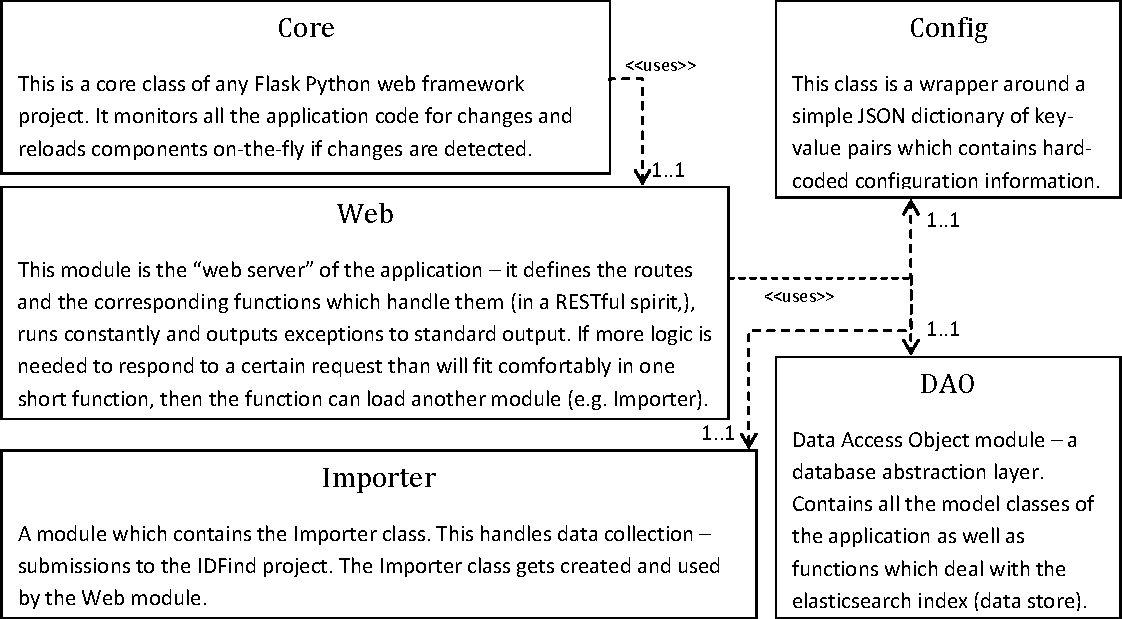
\includegraphics[width=1.00\textwidth,]{Chapter3/idfind-uml.pdf}
\caption{Overview of parent project IDFind's technical design presented in the Progress Report \cite{progress-report}}
\label{fig:idfind-uml}
\end{figure}

Figure \ref{fig:idfind-uml} was intended only as an overview and had intentionally left out

\section{Main Application}
\label{design-main-first}
% TODO remember to include classes contained within these modules in each module's description

\subsection{Core}
This is a core class of any Flask Python web framework project. It monitors all application code for changes and reloads components on-the-fly if changes are detected.

\subsection{DAO}
Data Access Object module – a database abstraction layer. Contains all the model classes of the application as well as functions which deal with the elasticsearch index (data store).

\subsection{Web}
This module is the ``web server'' of the application – it defines the routes and the corresponding functions which handle them (in a RESTful way), runs constantly and outputs exceptions to standard output. If more logic is needed to respond to a certain request than will fit comfortably in one short function, then the function can load another module (e.g. Importer).

\subsection{Importer}
A module which contains the Importer class. This handles data collection – submissions to the IDFind project. The Importer class gets created and used by the Web module.

\subsection{Config}
This class is a wrapper around a simple JSON dictionary of key-value pairs which contains hard-coded configuration information.

\subsubsection{Default Settings}

\subsection{Util}

\subsection{TweetBot}

\section{Suggestions}


\section{Harvesters}
\label{design-main-last}

\subsection{HarvesterBase}

\subsection{CliManualSubmitter}
% why break naming conventions for classes? well, BBSRCRSSHarvester..... so hard-line first-letter-only-capital. But then have to use same convention everywhere - so that's how it happened.

\subsection{RssHarvesterBase}

\subsubsection{BbsrcRssHarvester}

\subsubsection{EsrcRssHarvester}

\subsection{EmailHarvesterBase}

\subsubsection{EpsrcEmailHarvester}

\section{Datastore}
\label{design-datastore}
 Indexing software is usually most easily understood in comparison to more traditional approaches of storing data, like relational databases (MySQL \cite{mysql}, Oracle \cite{oracle}). These store data in a highly structured way and the base structural unit is a table (theoretically equivalent to a set, which is where relational theory and such databases come from). The ``indexing'' part actually means ``analysis'' in the broadest sense. Given data - any data, images, text, Microsoft Word binary blobs pretending to be text - the software will try to find common features or look for certain characteristics in the data. For example, it will try to discern whether a particular string actually represent a datetime value.
 
 Elasticsearch is actually a NoSQL datastore - which essentially means that it deals with very simple key-value pairs as the basic unit of organising data \emph{instead of} tables, or sets. It also supports slightly more complex, but still very simple structures, such as lists and dictionaries (a.k.a. HashMaps). This means that the storage representation is also quite simple - in this case, all documents stored within an elasticsearch instance can be represented in the JSON data format. This simplicity enables elasticsearch to deal with semistructured data much more easily than a traditional relational database.
 
 A lot of funding data can be considered semistructured - one type of funding call might have a closing date, another one might not. When multiple data sources are considered it becomes even more difficult since different organisations publish different bits of data about their available funding. Since elasticsearch combines its simple storage with a powerful, fast search engine this makes such ``holes'' in the data a lot less important than usual - the ``usefulness'' of the data scales with its quality (there is no getting around the fact that less holes is better), but \emph{the software can deal with it} without throwing null pointer exceptions and \emph{the data that is present is still easily discoverable}.
 
 % TODO REVIEW include an example of a JSON document that FundFind has, and then represent the same document using a relational structure of several tables. Point out how many are needed and that it's cumbersome. Concede that it gives a speed advantage with a lot of records, but retort that elasticsearch already achieves that speed just by searching the data instead of structuring it in a specific way, so the database can find it more quickly on disk...
 
 Elasticsearch's RESTful JSON-returning API usually enables rapid prototyping, evaluation and integration with Javascript visualisation libraries such as d3 \cite{d3} and BubbleTree \cite{bubbletree}. While these precise features are not implemented in this version of FundFind, the decision to use elasticsearch leaves this option open.
 
 % TODO ADD additionally, elasticsearch is asynchronous. Why the fuck is this an advantage over synchronous communication? Find text on this and re-write it here. Blocking for I/O, communicating with database usually a problem (caused meltdowns every year when marks were released). So maybe that's why it's better essentially.
 
 % TODO add backup procedures for elasticsearch - just copy the files. Although you can get all the data out via the API as well. Async may help here (backup not hogging connections?).

\section{User Interface}
% Looked at what values the data had in general, starting with EPSRC examples and some RSS feeds (cite them here).
% Bootstrap integrates a lot of UI knowledge into itself
% which is good, but not sufficient - reused IDFind's homepage design made by Mark @ Cottage Labs \cite{mark}.
% submission forms - just ordered the items in order of perceived importance, mostly as presented in EPSRC data and RSS feeds. Put things related to FundFind at the bottom (e.g. tags) since the best way to write such metadata is to have thought about the values in the rest of the form.
\subsection{AJAX functionality}
\label{design-ajax}
  %utilities e.g. slug
  %gtr advanced suggestion stuff

\section{API}
  % divide into ``usability design'' - how usable API is by developers, what thought was put into that
  % and technical design
  \subsection{Design for Developers}
    % general waffle
    % route table with explanations
    
    In addition to the functionality exposed through the routes described above, the AJAX functionality (\S\ref{design-ajax}) can also be used by API consumers. For example, the developers of a hypothetical ``News for Scholars'' newsfeed reader application might want to suggest previously funded bids to its UK readers. They have two options:
    
    \begin{enumerate}
     \item Re-use the classes within the Suggest module which enable FundFind's ``this may be of interest'' feature. If the hypothetical application is written in Python, this will just involve copying $+$ editing the code and perhaps reading the Gateway to Research API documentation (for the UK information). If it is written in another language, ``re-use'' will mean looking at the logic contained within the 
    \end{enumerate}

  \subsection{Technical design}
  \label{api-tech-design}
  % Intro - API achieved by relying on the usual Python technologies, Flask, whatever IDFind had as basic API..
  % Used HTTP protocol. What it is. Why.
  \subsubsection{Data format}
  % why JSON for the API - interoperability, cite stuff
  % JSON is used in the back-end anyway - FundFind itself uses it when communicating with elasticsearch
  % refer to \label{design-datastore}
  % conneg. integrated Richard's package?
 
\section{Alternative Designs}
\chapter{Implementation}

% The implementation should look at any issues you encountered as you tried to implement your design. During the work, you might have found that elements of your design were unnecessary or overly complex, perhaps third party libraries were available that simplified some of the functions that you intended to implement. If things were easier in some areas, then how did you adapt your project to take account of your findings?

% It is more likely that things were more complex than you first thought. In particular, were there any problems or difficulties that you found during implementation that you had to address? Did such problems simply delay you or were they more significant? Your implementation might well be described in the same chapter as Problems (see below).

% working within context of other projects, have to keep conventions in mind, although better ways of doing things always welcome
\section{User Interface}
\label{impl-ui}

\section{Implementing The Main Application}

\subsection{Faceted Search}
\label{impl-facetview}
% describe how searches can be shared just by copying the url of the search page

\subsection{The Final Features}

\subsubsection{Responsive Mobile Web Design}
\label{impl-mobile}

\subsection{The Dropped Features}
% TODO add all the dropped features from chapter 2, Initial Requirements here
The decision to drop some features came after some design and exploratory technical work had been done.

\subsubsection{Harvesting Funding Data From E-mail Digests}
\label{impl-email-parse}
\chapter{Testing}

% Detailed descriptions of every test case are definitely not what is required here. What is important is to show that you adopted a sensible strategy that was, in principle, capable of testing the system adequately even if you did not have the time to test the system fully.

% Have you tested your system on 'real users'? For example, if your system is supposed to solve a problem for a business, then it would be appropriate to present your approach to involve the users in the testing process and to record the results that you obtained. Depending on the level of detail, it is likely that you would put any detailed results in an appendix.

\section{Overall Approach to Testing}
% all testing except user testing automated

% pretty much the same content being tested in different ways
% so have unit and integration tests
% integration asserted content -> selenium for automated UI testing
% integration asserted content -> mechanize for automated stress testing

\section{Automated Testing}

\subsection{Unit Tests}
% based on bibserver setup

\subsection{Functional / Integration Tests}
% based on bibserver setup
% automated integration testing - after unit tests have succeeded, tests paths of functionality that use multiple modules

\subsection{User Interface Testing}
%selenuim ide

\subsection{Stress Testing}
% multi-mechanize

%\subsection{Other types of testing}

\section{User Testing}
% TODO WORK tested with candidate PG-s, PG-s, Postdocs, Lecturers, Developers
\chapter{Evaluation}

%Such material is regarded as an important part of the dissertation; it should demonstrate that you are capable not only of carrying out a piece of work but also of thinking critically about how you did it and how you might have done it better. This is seen as an important part of an honours degree. 

%There will be good things and room for improvement with any project. As you write this section, identify and discuss the parts of the work that went well and also consider ways in which the work could be improved. 

%The critical evaluation can sometimes be the weakest aspect of most project dissertations. We will discuss this in a future lecture and there are some additional points raised on the project website. 

\section{Approaching the field of scholarly funding}
\label{eval-difficult-field}
% amorphous, ill-defined
% possible to achieve automation and great time/cost savings but will need consensus from funders
% fundees will follow, but funders want to be careful when making changes - not drive away good researchers who can do the job
% FundFind can be developed further to facilitate this - show funders the benefits of agreeing on a common representation of their data, show fundees the benefits of being able to search transparently across organisations
% FIXME
Somewhere in February, the 4th (out of 6) month of the project, I realised that this domain of knowledge, scholarly funding, was going to be a tougher nut to crack than I had thought.

decided late that the project was going to do requirements gathering as a formalised goal - inspired both by G4HE (Cottage Labs project) and difficulties in understanding the field \S\ref{eval-difficult-field}. These only became clear once the technical work started in earnest and it turned out it was in fact both a pretty big field, and one that was ripe with problems and conflicting interests.

TODO FIXME EXPAND THIS HERE INTO A SUBSECTION ABOUT WHAT LEARNED ABOUT FIELD. Regardless of personal interest, it takes time to develop holistic understanding of a field like this. One analogy would be another human field of endeavour the author has a personal interest in - saving and re-homing homeless animals. Ripe with conflicting interests with a troubled history of ad-hoc evolution resulting from the intersection of these interests. FIXME TODO EXPAND HERE exactly what are the problems? Politics, money and the sincere wish to save every animal encountered, the good intentions sometimes resulting in bad outcomes 
such as houses full of tens of animals which cannot be taken care of.

% FIXME
Relating information about the field and its problems to people outside the target audience and even across target user groups turned out to be much more difficult than expected. TODO more here?

\subsection{Condensing the insights gained}
Part of the point of the project was to see how the funding field worked. And this went fine, I now know a lot more about it than when I started. However, sharing this information seems really difficult. It feels like my sample was way too small and that any representation I choose for it will just be laughably bad. In reality, there is clearly a place in the world for a ``how does scholarly funding work for beginners, from a beginner'' collection of information, but presenting this appropriately seems incredibly difficult.

All the insights gained were attained through interviews. However, it was just my opinion of the content of these meetings that was actually going to make it into the final output. This can feel quite daunting - as a developer, I prefer to publish the data and let those whose work I support actually ``deal'' with it. However, in this case, I \emph{am} the researcher, this mysteriously skilled person who somehow knows what to do with this data. Others do not want to know about conversations I have had, they want knowledge - even understanding. My understanding. % TODO expand this

%However, I have done similar things before - I talked about what Open Knowledge is while I was still figuring it out, so I decided late on that one of the outputs of this project was to be a blog post on the topic. My previous attempt to tackle a new field is published on the Cottage Labs website, and we do publish thoughts which concern the Higher Education field, so this seemed like a good place to publish it \cite{fundfind-blog-post}.
% FOR THE ABOVE ^ - NOTE chapter 1 has a relevant to-do item should I have some outputs which ``distill'' this knowledge? Like a blog post on the CL website, or publish a list of the features or the progression of FundFind features, or just a blog post about FundFind dev process?

\section{Collecting Information From Disparate Sources - Technological Suitability}
% Were the design decisions correct?
% Could a more suitable set of tools have been chosen?
% design decisions - evaluated
% better tools, better decisions possible?

\section{User Needs}
\subsection{Identifying Requirements}
% Were the requirements correctly identified? 
Far too much thought seems to have been given to the priority of features - at the end it's just a list of functions and they're all desirable. There was not a single feature which was later identified as a ``bad'' idea. Of course, they can be roughly grouped according to what users seemed to want and this is very important in guiding future development, but in hindsight, there does not seem to be much value in the detailed prioritisation presented in \myref{initial-reqs}. With rough groups such as ``vital'', ``desirable'', ``low priority'', the prioritisation process could be simplified significantly and there would be relatively few features that would be difficult to categorise.

It was still sensible to categorise new features which came up during development, since the feature list was not really fixed until development had ended.

\subsection{Meeting Needs}
% How well did the software meet the needs of those who were expecting to use it?
% not about features, but data

\subsubsection{Those Looking To Analyse Scholarly Funding}

\subsubsection{Exploring Scholarly Funding}
Within the group of people with analytical needs, there was a sub-group of developers which inspired and was part of the reason the project was conceived - Cottage Labs LLP, the Open Knowledge Foundation and the author. It was always the project's intention to learn about scholarly funding specifically so that these people could have a better idea of how to meet the Higher Education sector's needs.
% How well were any other project aims achieved?
% learn more about it
% personally, Cottage Labs, OKFN, Open Knowledge movement

\section{In Retrospect}
% If you were starting again, what would you do differently?

% chapter 2 says Basing the project on another one that the author had participated in meant that a great deal of bootstrapping time was saved. A lot of knowledge about using the underlying Python frameworks was also reused. On the other hand, trying to create something to the standards enforced by other projects in the same context (Open Knowledge) forced quite a lot of reading that might not have been strictly necessary outside this context.

% BUT it took quite a while to extend that knowledge to make the frameworks do what I wanted them to do NOW.
% About 2nd sentence - trying to make something up to a certain standard that I hadn't coded to before was certainly difficult. The years of experience some of the authors of these projects have certainly have an impact on how quickly they seem to be able to write quality code. On the other hand, that is one of the great things about the Open Knowledge field, as long as it showcases a worthwhile idea and you spend enough time on it, it will gain at least recognition, and probably traction.

% On the other hand, quite a lot of time went into actually learning to use the new editor.
% so was it a good idea? used for all other programming projects throughout the year so it was not strictly a decision within the project, but don't think not doing it would have saved a great amount of time

\section{Future Work}
\label{future-work}
% what
% why not included in this project's scope
% why is it interesting

% talk about all dropped features? group them in what ways they could be used? or maybe make it feature-centric since some of them can be used in different ways

% chapter 1 says Identify user requirements in the funding sector. Results presented in \myref{audience} above and more concretely in \myref{devprocess-requirements}. The data must be sufficient to enable the creation of a project roadmap for a) future research work into the requirements of user groups which were not engaged during this project; b) concrete development work which would build on the software built during this project. The foundations for this are laid in presented in \myref{future-work}.

\subsubsection{E-mail Alerts}
This is a good feature and it's great that it was identified, especially since the author was not previously aware of the current scholars' workflow.

%research officers' reports \myref{audience-research-officers}).
\label{future-research-officers-reports}

\subsubsection{Exporting The Results Of Searches}
Nonetheless, research development officers' reports mentioned in \myref{audience-research-officers} could benefit from this feature, so it was added to Future Work, \myref{future-work}.

% feedback option

% use the tagging and profile information in ANY way
% e.g. browse tags

\section{Learning}
% LaTeX skills - not in industry, but if ever return to academia, lots of useful learned. Wordcount script, macros, large documents, divide focus using chapter files.
% Open Knowledge field
% funding field
% Python for web applications, specifically in the way it's used by future employer
%\chapter{Example \LaTeX}

This chapter includes some example \LaTeX. 

Ever advancing developments in computational power... mean ever more pictures
of kittens on the internet. As you will see in Figure~\ref{fig:kittenpicture},
some of them are very cute.

\begin{figure}[H]
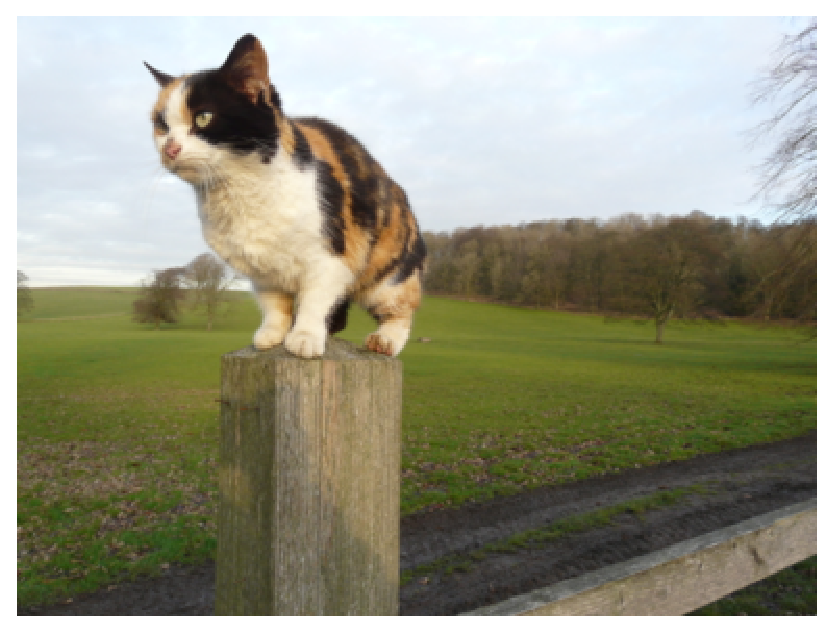
\includegraphics{Chapter7/kitten}
\caption{A picture of a kitten\cite{kittenpic_ref}.}
\label{fig:kittenpicture}
\end{figure}

\section{Overview}

In this section I am going to include a spurious label\label{spurious}, which
appears in the code but has no effect on the display at the time it was
inserted.  I am also going to include a spurious citation to a journal
article \cite{HannahsPaper}, a citation to a conference paper \cite{MarksPaper},
a citation to a book \cite{NumericalRecipes}, and a citation to a
website \cite{FailBlog}. All of these citations have been added to the BibTeX
(.bib) file which you'll find in the References directory -- they include some
tricky stuff (accents and so on) which are explained in the comments in the
BibTeX.


\subsection{A bit of extra text to give the section some bulk}

This is a paragraph of extra text just to make this section go over into a
second page and to show the use of headers and page numbering that happens
automatically once the text flows over to another page.  

\section{A few words of advice on \LaTeX}

One thing you should be aware of using \LaTeX\ is that \LaTeX\ has its own
ideas about where things should be placed and about where page breaks should
happen.  This minimises the chances of widow and orphan
text\footnote{\emph{Orphan} and \emph{Widow} text are when the last line of a
paragraph appears on the following page, or where a header appears on one page
and the following text appears on the next}, but it can lead to you feeling
like you've lost control if you're used to using software like Word.  The best
advice for text formatting is to just relax and relinquish control to \LaTeX;
for figures, it's a good idea to use the float package (already included in
this template) and put [H] after your includegraphics command.  You can see an
example of this usage in the code used to insert Figure~\ref{fig:kittenpicture}
on Page~\pageref{fig:kittenpicture}.

In the following paragraph, I've put a pointless equation. This is just so that you can see how to include an equation in a document. Equations are numbered separately, just like tables and figures.

\begin{equation}
X=\sum_{i=1}^{N} x_{i}+y_{i}
\label{eq:spurious}
\end{equation}

Like tables and figures, if you label an equation you can refer back to it
using the ref command (for the number of the equation) or the pageref command
(for the page the equation lies on).  The source for this document has examples
of both types of reference here: Equation~\ref{eq:spurious} lies on
Page~\pageref{eq:spurious}.

\section{Early work}

\begin{table}[H]
\begin{tabular}{l c l}
Year & Kitten frequency & Notes \\
\hline
1993 & 0.04& World wide web begins to become popular \\
1995 & 0.2 & Kittens take over\\
2008 & 0.34 & Cats make a stand\\
\end{tabular}
\caption{A pointless table, inserted to show that the list of tables will auto-update}
\end{table}

\subsection{The first signs of this topic}

In this section we have a spurious link back to a spurious label, which appeared in Section~\ref{spurious}.

% the use of ~ is a space that will not break over a line - use it
% after Section and Chapter to make sure it looks tidy





% add any additional chapters here

\setemptyheader
\addcontentsline{toc}{chapter}{Appendices}
\chapter*{Appendices}
\pagebreak

% start the appendix - sets up different numbering
\fancypagestyle{plain}{%
%\fancyhf{} % clear all header and footer fields
\fancyhead[L]{\textsl{Appendix\ \thechapter}}
\fancyhead[R]{\textsl{\leftmark}}}

\appendix
\fancyhead[L]{\textsl{Appendix\ \thechapter}}
\fancyhead[R]{\textsl{\leftmark}}
\fancyhead[C]{}
\fancyfoot[C]{\thepage}
\renewcommand{\headrulewidth}{0.4pt}
\renewcommand{\chaptermark}[1]{\markboth{#1}{}}

\fancyhead[L]{\textsl{Appendix\ \thechapter}}
\fancyhead[R]{\textsl{\leftmark}}
\fancyfoot[C]{{\thepage} of \pageref{LastPage}}

% include any appendices here
\chapter{Third-Party Code and Libraries}
\label{third-party}

\section{FundFind}
\subsection{Python Packages}
\subsubsection{Python Standard Distribution Packages}
|json| is used for parsing the JSON data format (e.g. the app configuration is in a JSON file, the API responds with JSON).

|sys| and |os| are Python packages for interacting with the Operating System. |sys| contains certain global pieces of information such as the running Python version number.

|logging| handles logging output such as warnings, errors or just debugging information to the command line and to files.

|uuid| handles the generation of UUID-format unique identifiers.

|UserDict|, when subclassed by an application class, gives that class most of the properties of a dictionary. All |fundfind.dao| objects have property since they inherit from 
\\|fundfind.dao.DomainObject| which in turn is a child of |UserDict|. This allows things like |account['department']|.

|httplib| is one of the myriad of Python libraries for handling HTTP connections. |requests| is another one, albeit much cleaner and easier to use and is used in the FundFind tests. |httplib| is used by certain |dao| methods for accessing the datastore which were not changed from the parent IDFind codebase and can probably be refactored out of use by making more extensive use of the |pyes| elasticsearch access library.

|datetime| handles time in Python.

|re| is the standard regular expressions Python module.

|unicodedata| lends a hand in handling Unicode characters to the |util| module when producing URL-friendly slugs of strings.

\subsubsection{Other Python Packages}

Flask (|flask| in imports) is the main back-end framework upon which the whole web application is based \cite{flask}. The |fundfind.dao| module imports |werkzeug|, which is the underlying web server component for Flask for help with generating user password hashes.

The Flask-Login extension (|flask.ext.login| in imports) was used for helping with user authentication \cite{flask-login}. It does not provide registration capabilities or creating profiles.

|pyes| was used for connecting to elasticsearch datastore \cite{pyes}.

|parsedatetime| \cite{parsedatetime} is a module which tries to guess the time and date format from a simple string.

\subsection{Non-Python Code}
Web user interface libraries - Bootstrap \cite{bootstrap}, jQuery \cite{jquery}, jQuery UI \cite{jquery-ui}, linkify \cite{linkify} (linkify is just a jQuery plugin which turns text on HTML pages that looks like a URL into an actual clickable URL).

Search page - facetview \cite{facetview}, developed as a jQuery plugin.


\section{Funding Harvest}
Funding Harvest uses the standard distribution Python packages |datetime|, |logging|, |json|, |sys|, |uuid|, |UserDict| and |httplib|, described above, for the same reasons (mostly |config| and |dao| modules, which are very similar to FundFind's). It also uses |copy|, which a standard module which allows deep copies of objects to be made (i.e. when copying complex objects the actual values are copied, not just pointers to other objects, no matter how complex the hierarchy).

It does use one third-party (not a Python standard) module - feedparser \cite{feedparser} for parsing RSS feeds.

\chapter{File Listings}
\label{file-listings}

This Appendix provides a listing of all files in the source code repositories of |fundfind|, the main web application, and |fundingharvest|, the additional funding data harvesting project.

Its aim is to aid source code review and deeper understanding of the projects' technical details.

%TODO this
(Note: need to figure out how to get |tree -d|'s output in here and leave a short comment against each file.)

\section{fundfind}

\section{fundingharvest}

\fancypagestyle{plain}{%
   \fancyhead{} %[C]{Annotated Bibliography}
   \fancyfoot[C]{{\thepage} of \pageref{LastPage}} % except the center
   \renewcommand{\headrulewidth}{0pt}
   \renewcommand{\footrulewidth}{0pt}
}

\setemptyheader

\nocite{*} % include everything from the bibliography, irrespective of whether it has been referenced.

% the following line is included so that the bibliography is also shown in the table of contents. There is the possibility that this is added to the previous page for the bibliography. To address this, a newline is added so that it appears on the first page for the bibliography. 
\addcontentsline{toc}{chapter}{Annotated Bibliography} % Adds References to contents page

%
% example of including an annotated bibliography. The current style is an author date one. If you want to change, comment out the line and uncomment the subsequent line. You should also modify the packages included at the top (see the notes earlier in the file) and then trash your aux files and re-run. 
\bibliographystyle{authordate2annot}
%\bibliographystyle{IEEEannot}
\renewcommand{\bibname}{Annotated Bibliography} 
\bibliography{References/references} % References file


\end{document}
